\documentclass[12pt,fleqn]{article}\usepackage{../../common}
\begin{document}
Ders 1-8

Yaylar ve Agirliklar (Springs and Masses)

Dersimizin uygulama kismina geldik. Diyelim ki alttaki gibi bir yay sistemi var,
4 tane yay 3 tane agirliktan olusuyor, ve sonlari duvar, tavan gibi bir yerde
sabitlenmis.

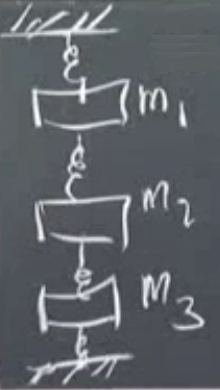
\includegraphics[width=5em]{compscieng_1_08_01.png}

Kutlelerin bir agirligi var tabii, agirliklar o yaylar asagi dogru cekiyor, bu
cekim yaylari acacak, gerecek, soru yaylarin ne kadar asagi inecegi.  Bir yer
degisim (displacement) sorusu bu yani. Unutmayalim yay acilip kapanan bir
mekanizmadir ama acilirken de kapanirken de bir direnc gosterir. Yer degisim en
ustte ve en altta sifir cunku oralar sabitlenmis.

Bir baslangic hali dusunursek, diyelim ki yercekimi o anda etkisiz, ama sonra
yercekimini bir dugmeye basip aciyoruz, her yay baslangic halinden asagi
dogru bir yer degisimi yasayacak, 

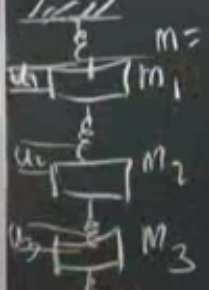
\includegraphics[width=5em]{compscieng_1_08_02.png}

bunlara $u_1,u_2,u_3$ diyebiliriz.

Dikkat salinimi olcmeye ugrasmiyoruz burada, o daha sonraki derslerde devreye
girecek, zaman faktorunu resme dahil edecegiz, o sonra. Simdi sadece kalici
durumla ilgileniyorum, yercekimi aciliyor, yaylar asagi dogru uzuyor, ve her sey
yerli yerine oturduktan sonra gozlemlenecek yer degisimiyle ilgileniyorum su
anda.

Ana denklem neye benzeyecek o zaman? Ilk agirlik mesela asagi inerken ilk yayi
gerecek. Hooke Kanunu bu noktada der ki yay belli bir kuvvetle agirligi geri
cekecek, bu cekis yayin gerilmesi / uzamasiyla orantili olacak.

Simdi dusunelim acaba mesela ikinci yay ne kadar uzar? $u_2-u_1$ kadar. Bir
farktan bahsediyoruz burada. Bazi yaylar sikisma da yasayabilir, mesela
tahmin ediyorum ki en alttaki yay sikisacak. 















[devam edecek]

\end{document}
